\documentclass[12pt,notitlepage]{article}
\usepackage[utf8]{inputenc}
\usepackage{natbib}
\usepackage[dutch]{babel}
\usepackage{graphicx}

\usepackage{blindtext}
\usepackage[final]{pdfpages}
\usepackage[a4paper, total={6.3in,9in},footskip=76pt]{geometry}


% make section start with Alphabet letters
\renewcommand{\thesection}{\alph{section}}

% plots
\usepackage{pgfplots}
\pgfplotsset{compat=1.8}
\pgfplotsset{mystyle/.style={%
        width=6in,
        ylabel={Tijd in milliseconden},
        xlabel={Aantal studenten},
        xmin=0,xmax=1280000,
        scaled y ticks = false,
        scaled x ticks = false,	
       	x tick label style={rotate=45, anchor=north east, inner sep=0mm},
       	legend pos=north west
        }}


\usepackage{titlesec}
\titlespacing\section{0pt}{12pt plus 4pt minus 2pt}{0pt plus 2pt minus 2pt}
\titlespacing\subsection{0pt}{0pt plus 4pt minus 2pt}{0pt plus 2pt minus 2pt}
\titlespacing\subsubsection{0pt}{12pt plus 4pt minus 2pt}{0pt plus 2pt minus 2pt}

% turn off word breaking
\usepackage{hyphenat}
\hyphenpenalty 10000
\exhyphenpenalty 10000
\raggedright

% make paragraphs with line spacing
\setlength{\parskip}{\baselineskip}%
\setlength{\parindent}{0pt}%


% Set up code listings for Java
\usepackage{listings}
\usepackage{color}

\definecolor{dkgreen}{rgb}{0,0.6,0}
\definecolor{gray}{rgb}{0.5,0.5,0.5}
\definecolor{mauve}{rgb}{0.58,0,0.82}

\lstset{frame=tb,
  language=Java,
  aboveskip=3mm,
  belowskip=3mm,
  showstringspaces=false,
  columns=flexible,
  basicstyle={\small\ttfamily},
  numbers=none,
  numberstyle=\tiny\color{gray},
  keywordstyle=\color{blue},
  commentstyle=\color{dkgreen},
  stringstyle=\color{mauve},
  breaklines=true,
  breakatwhitespace=true,
  tabsize=3
}

\begin{document}


%----------------------------------------------------------------------------------------
%	ONDERZOEKSVOORSTEL
%----------------------------------------------------------------------------------------

\begin{titlepage}

\newcommand{\HRule}{\rule{\linewidth}{0.5mm}}

\center % Center everything on the page

%----------------------------------------------------------------------------------------
%	HEADING SECTIONS
%----------------------------------------------------------------------------------------
\begin{figure}[h!]
\centering
\includegraphics[scale=0.5]{hva-logo.png}
\end{figure}
\textsc{\LARGE Hogeschool van Amsterdam}\\[1.5cm] % Name of your university/college
\textsc{\Large Sorting \& Searching}\\[0.5cm] % Major heading such as course name
\textsc{\large Efficiëntie van geavanceerde sorteeralgoritmes}\\[0.5cm] % Minor heading such as course title

%----------------------------------------------------------------------------------------
%	TITLE SECTION
%----------------------------------------------------------------------------------------

\HRule \\[0.4cm]
{ \huge \bfseries Practicum 1}\\[0.2cm] % Title of your document
\HRule \\[1.2cm]

% Optimalisatie van gegevensverwerking voor iLocate

%----------------------------------------------------------------------------------------
%	AUTHOR SECTION
%----------------------------------------------------------------------------------------

\begin{minipage}{0.4\textwidth}
\begin{flushleft} \large
\emph{Author:}\\
Robert \textsc{Bakker} % Your name
\linebreak
\linebreak
\emph{Studentnummer:}\\
500689284
\linebreak
\linebreak
\emph{Klas:}\\
IVSE4

\end{flushleft}
\end{minipage}
~
\begin{minipage}{0.4\textwidth}
\begin{flushright} \large
\emph{Author:}\\
Mark \textsc{van der Steenhoven} % Your name
\linebreak
\linebreak
\emph{Studentnummer:}\\
500693745
\linebreak
\linebreak
\emph{Klas:}\\
IVSE4
\end{flushright}
\end{minipage}\\[4cm]

%----------------------------------------------------------------------------------------
%	DATE SECTION
%----------------------------------------------------------------------------------------

{\large Blok 2, 2016 - 2017}\\[3cm] % Date, change the \today to a set date if you want to be precise

%----------------------------------------------------------------------------------------
%	LOGO SECTION
%----------------------------------------------------------------------------------------

%\includegraphics{Logo}\\[1cm] % Include a department/university logo - this will require the graphicx package

%----------------------------------------------------------------------------------------

\vfill % Fill the rest of the page with whitespace

\end{titlepage}


%----------------------------------------------------------------------------------------
%	TABLE OF CONTENTS
%----------------------------------------------------------------------------------------
\renewcommand{\contentsname}{Inhoudsopgave}
\tableofcontents
\clearpage

%----------------------------------------------------------------------------------------
%	Opdracht a
%----------------------------------------------------------------------------------------

\section{Resultaten van studenten sorteren met een advanced sort}
Voor deze opdracht wordt gebruik gemaakt van de volgende Student-klasse:

\begin{lstlisting}
public class Student implements Comparable<Student> {

    private String group;
    private int studentNumber;
    private float grade;

    public Student(String group, int studentNumber, float grade) {
        this.group = group;
        this.studentNumber = studentNumber;
        this.grade = grade;
    }
    
    // Getters and Setters
    
    @Override
    public int compareTo(Student that) {
        if (this.grade < that.getGrade()) return 1;
        if (this.grade > that.getGrade()) return -1;
        if(this.studentNumber > that.getStudentNumber()) return -1;
        if(this.studentNumber < that.getStudentNumber()) return 1;

        return 0;
    }
}
\end{lstlisting}

Waarbij het met name gaat om de implementatie van de Comparable-interface. Als twee Student-objecten met elkaar worden vergeleken, wordt in eerste instantie gekeken naar het cijfer (grade). Mochten de cijfers niet groter of kleiner zijn dan elkaar oftwel gelijk zijn, wordt er teruggevallen op een vergelijking op het studentnummer.

\clearpage
\subsection{Quicksort implemenatie}
Hieronder de Quicksort implementatie voor de experimenten in paragraaf a.2 met zoveel mogelijk uitleg in het codecommentaar:
\begin{lstlisting}

    // De quicksort accepteert een lijst van objecten met een Comparable
    // interface (bijv. de Student-klasse), het beginpunt vanaf links,
    // en het beginpunt vanaf rechts 
    private void quicksort(Comparable[] list, int low, int high) {

        // Neem het middelpunt van de array als spil (draaipunt)
        Comparable pivot = list[low + (high - low) / 2];

        int i = low; // linkerkant
        int j = high; // rechterkant

        while (i <= j) {
            // Wanneer object vanaf links kleiner is dan de spil
            // Verschuif naar de volgende in de linkerlijst
            while (list[i].compareTo(pivot) < 0) i++;

            // Wanneer object vanaf rechts groter is dan de spil
            // Verschuif naar de volgende in de rechterlijst
            while (list[j].compareTo(pivot) > 0) j--;

            // Als er een index van de linkerlijst is gevonden, met een waarde
            // die groter is dan de spil, en een index in de rechterlijst met
            // een waarde die kleiner is dan de spil, moeten de 2 waarden
            // worden omgedraaid
            if (i <= j) {
                Comparable temp = list[i];
                list[i] = list[j];
                list[j] = temp;
                i++;
                j--;
            }
        }
        // Hetzelfde voor de rest van de linkerlijst
        if (low < j) {
            quicksort(list, low, j);
        }
        // en voor de rechterlijst
        if (high > i) {
            quicksort(list, i, high);
        }
    }
\end{lstlisting}

\clearpage
\subsection{Resultaten experiment}
Het experiment bestond uit het meten van de tijd die de Quicksort implementatie in de vorige paragraaf nodig heeft om lijsten met verschillende aantallen studenten te sorteren.

Om meetresultaten accurater te maken werd Java met de VM optie \textsf{-Djava.compiler=NONE} uitgevoerd om optimalisaties uit te schakelen. Die optie voorkomt dat Java het programma met extra optimalisaties gaat uitvoeren, wat anderszijds invloed zou hebben op de meetresultaten.

\begin{lstlisting}
int[] numberOfStudents = {10000, 20000, 40000, 80000, 
160000, 320000, 640000, 1280000};
// N_EXPERIMENTS = 5
long[][] quicksortResults = new long[numberOfStudents.length][N_EXPERIMENTS]; 

for (int i = 0; i < numberOfStudents.length; i++) {
    for (int j = 0; j < N_EXPERIMENTS; j++) {
        ResultList list = StudentListGenerator.generate(numberOfStudents[i]);
        list.shuffle(); // StdRandom.shuffle()
        long startTime = System.currentTimeMillis();
        list.quicksort(); // De Quicksort implementatie
        long endTime = System.currentTimeMillis();
        quicksortResults[i][j] = (endTime - startTime);
    }
}
\end{lstlisting}

Het experiment is meerdere keren uitgevoerd en daarvan is het gemiddelde genomen. Dit zijn de resultaten:

\begin{center}
\begin{table}[htb]
\begin{tabular}{| l | l | l | l | l | l | l |}
\hline
Aantal studenten & Run 1 & Run 2 & Run 3 & Run 4 & Run 5 & Gemiddelde\\ \hline
10000 & 44 & 31 & 27 & 30 & 30 & 32\\ \hline
20000 & 64 & 61 & 66 & 66 & 66 & 64\\ \hline
40000 & 139 & 137 & 143 & 127 & 128 & 134\\ \hline
80000 & 291 & 288 & 337 & 301 & 329 & 309\\ \hline
160000 & 665 & 661 & 673 & 635 & 692 & 665\\ \hline
320000 & 1478 & 1427 & 1408 & 1422 & 1433 & 1433\\ \hline
640000 & 3045 & 3339 & 3059 & 3022 & 3128 & 3118\\ \hline
1280000 & 7085 & 6897 & 7003 & 8066 & 6974 & 7205\\ \hline
\end{tabular}
\end{table}
\end{center}

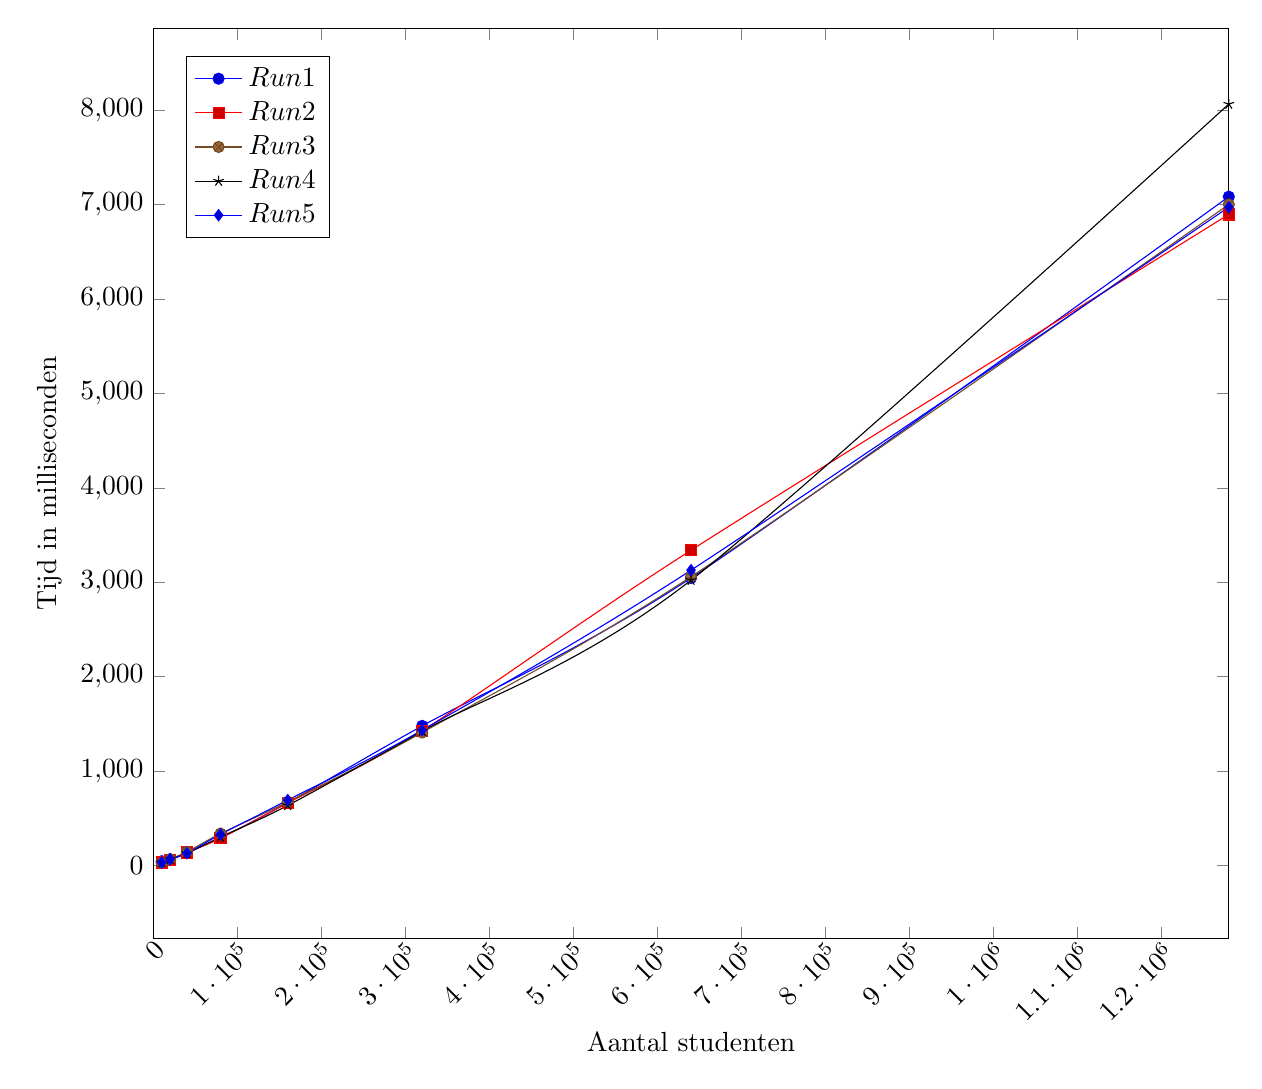
\begin{tikzpicture}
  \begin{axis}[mystyle]
\addlegendentry{$Run 1$}
\addplot+[smooth] coordinates
{(10000, 44) (20000, 64) (40000, 139) (80000, 291) (160000, 665) (320000, 1478) (640000, 3045) (1280000, 7085) };
\addlegendentry{$Run 2$}
\addplot+[smooth] coordinates
{(10000, 31) (20000, 61) (40000, 137) (80000, 288) (160000, 661) (320000, 1427) (640000, 3339) (1280000, 6897) };
\addlegendentry{$Run 3$}
\addplot+[smooth] coordinates
{(10000, 27) (20000, 66) (40000, 143) (80000, 337) (160000, 673) (320000, 1408) (640000, 3059) (1280000, 7003) };
\addlegendentry{$Run 4$}
\addplot+[smooth] coordinates
{(10000, 30) (20000, 66) (40000, 127) (80000, 301) (160000, 635) (320000, 1422) (640000, 3022) (1280000, 8066) };
\addlegendentry{$Run 5$}
\addplot+[smooth] coordinates
{(10000, 30) (20000, 66) (40000, 128) (80000, 329) (160000, 692) (320000, 1433) (640000, 3128) (1280000, 6974) };

  \end{axis}
\end{tikzpicture}
\clearpage
\subsection{Efficiëntie}

t is de gemiddelde tijd per aantal studenten n. Hier berekenen de gemiddelde factor waarmee de tijd groeit als het aantal studenten verdubbelt:

\begin{center}
\begin{table}[htb]
\begin{tabular}{| l | l |}
\hline
t & t+1 / t \\ \hline
32 & - \\ \hline
64 & 64/32 = 2 \\ \hline
134 & 134/64 = 2.093 \\ \hline
309 & 309/134 = 2.306 \\ \hline
665 & 665/309 = 2.152 \\ \hline
1433 & 1433/665 = 2.154 \\ \hline
3118 & 3118/1433 = 2.176 \\ \hline
7085 & 7085/3118 = 2.272 \\ \hline
\end{tabular}
\end{table}
\end{center}

Bij verdubbeling van het aantal studenten wordt de tijd gemiddeld:

(2+2.093+2.306+2.152+2.154+2.176+2.172) / 7 = 2.15042857143

zo groot.

(2 log 2.15042857143) / (2 log 2) = 1.10462421156...

2^{1.10462421156} = 2.15042857143

Als in de tabel te zien, wanneer n (aantal studenten) verdubbeld, verdubbeld ongeveer de tijd ook mee.

De Big-O is ongeveer O(n^{1.10462421156})	

%----------------------------------------------------------------------------------------
%	Opdracht b
%----------------------------------------------------------------------------------------
\section{Verbetering toevoegen aan algoritme}

\subsection{Experiment}

Hetzelfde als het vorige experiment, maar dan met het Median-of-3 algoritme vanuit het boek.

\begin{center}
\begin{table}[htb]
\begin{tabular}{| l | l | l | l | l | l | l |}
\hline
Aantal studenten & Run 1 & Run 2 & Run 3 & Run 4 & Run 5 & Gemiddelde\\ \hline
10000 & 67 & 33 & 30 & 29 & 34 & 38\\ \hline
20000 & 82 & 67 & 61 & 75 & 68 & 70\\ \hline
40000 & 146 & 149 & 150 & 158 & 158 & 152\\ \hline
80000 & 384 & 363 & 324 & 333 & 341 & 349\\ \hline
160000 & 689 & 730 & 738 & 727 & 787 & 734\\ \hline
320000 & 1918 & 2452 & 1642 & 2040 & 2504 & 2111\\ \hline
640000 & 4586 & 4493 & 3543 & 3555 & 3480 & 3931\\ \hline
1280000 & 7865 & 7915 & 8285 & 8178 & 8754 & 8199\\ \hline
\end{tabular}
\end{table}
\end{center}

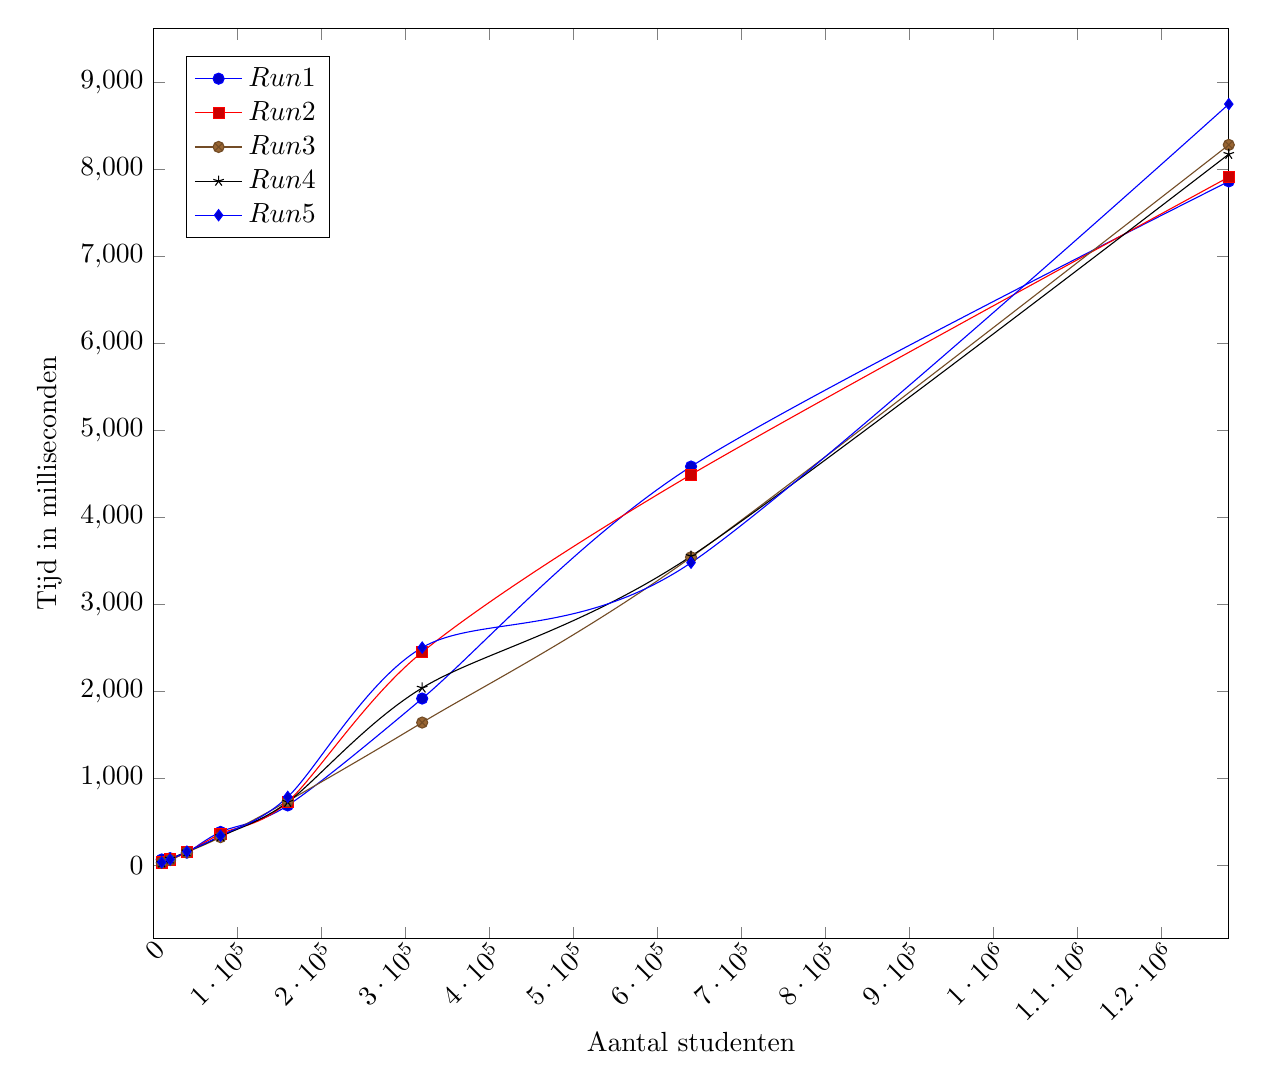
\begin{tikzpicture}
  \begin{axis}[mystyle]
\addlegendentry{$Run 1$}
\addplot+[smooth] coordinates
{(10000, 67) (20000, 82) (40000, 146) (80000, 384) (160000, 689) (320000, 1918) (640000, 4586) (1280000, 7865) };
\addlegendentry{$Run 2$}
\addplot+[smooth] coordinates
{(10000, 33) (20000, 67) (40000, 149) (80000, 363) (160000, 730) (320000, 2452) (640000, 4493) (1280000, 7915) };
\addlegendentry{$Run 3$}
\addplot+[smooth] coordinates
{(10000, 30) (20000, 61) (40000, 150) (80000, 324) (160000, 738) (320000, 1642) (640000, 3543) (1280000, 8285) };
\addlegendentry{$Run 4$}
\addplot+[smooth] coordinates
{(10000, 29) (20000, 75) (40000, 158) (80000, 333) (160000, 727) (320000, 2040) (640000, 3555) (1280000, 8178) };
\addlegendentry{$Run 5$}
\addplot+[smooth] coordinates
{(10000, 34) (20000, 68) (40000, 158) (80000, 341) (160000, 787) (320000, 2504) (640000, 3480) (1280000, 8754) };

  \end{axis}
\end{tikzpicture}
\clearpage

\subsection{Efficiëntie}

t is de gemiddelde tijd per aantal studenten n. Hier berekenen de gemiddelde factor waarmee de tijd groeit als het aantal studenten verdubbelt:

\begin{center}
\begin{table}[htb]
\begin{tabular}{| l | l |}
\hline
t & t+1 / t \\ \hline
38 & - \\ \hline
70 & 70/38 = 1.842 \\ \hline
152 & 152/70 = 2.171 \\ \hline
349 & 349/152 = 2.296 \\ \hline
734 & 734/349 = 2.103 \\ \hline
2111 & 2111/734 = 2.876 \\ \hline
3931 & 3931/2111 = 1.862 \\ \hline
8199 & 8199/3931 = 2.085 \\ \hline
\end{tabular}
\end{table}
\end{center}

Bij verdubbeling van het aantal studenten wordt de tijd gemiddeld:

(1.842+2.171+2.296+2.103+2.876+1.862+2.085)/7 = 2.17642857143

zo groot.

(2 log 2.17642857143) / (2 log 2) = 1.12196267286...

2^{1.12196267286} = 2.17642857143

Als in de tabel te zien, wanneer n (aantal studenten) verdubbeld, verdubbeld ongeveer de tijd ook mee.

De Big-O is ongeveer O(n^{1.12196267286})

Verwaarloosbaar verschil met het vorige experiment.

\clearpage
%----------------------------------------------------------------------------------------
%	Opdracht c
%----------------------------------------------------------------------------------------
\section{Resultaten in een Binary Search Tree en implementatie van rank()}

\subsection{Duplicaten}
Om duplicaten(studenten met hetzelfde cijfer) in de BST te kunnen plaatsen, krijgt de Node binnen de BST in plaats van 1 waarde, een lijst van waardes:

\begin{lstlisting}
private class Node {

    private Key key;
    private List<Value> val = new LinkedList<Value>(); // Lijst i.p.v. alleen Value
    private Node left, right;
    private int N;

    public Node(Key key, Value val, int N) {
        this.key = key;
        this.val.add(val); // Voeg toe aan lijst
        this.N = N;
    }
}
\end{lstlisting}

Het probleem met de implementatie uit het boek is dat wanneer, via de put() methode, er 2 Nodes worden toegevoegd met dezelfde Key, de Value wordt overschreven. Dit is opgelost door het aan de List toe te voegen:

\begin{lstlisting}
private Node put(Node x, Key key, Value val) {
    if (x == null) {
        return new Node(key, val, 1);
    }
    int cmp = key.compareTo(x.key);
    if (cmp < 0) {
        x.left = put(x.left, key, val);
    } else if (cmp > 0) {
        x.right = put(x.right, key, val);
    } else {
        // Voeg toe aan lijst i.p.v. overschrijven single value
        x.val.add(val); 
    }
    x.N = size(x.left) + size(x.right) + 1;
    return x;
}
\end{lstlisting}
\clearpage
En de get() method geeft nu in plaats van 1 waarde, een lijst terug:

\begin{lstlisting}
private List<Value> get(Node x, Key key) {
    if (x == null) {
        return null;
    }
    int cmp = key.compareTo(x.key);
    if (cmp < 0) {
        return get(x.left, key);
    } else if (cmp < 0) {
        return get(x.right, key);
    } else {
        return x.val;
    }
}
\end{lstlisting}

\subsection{Rank()}
\subsubsection{BST implementatie rank()}

\begin{lstlisting}

 private int rank(Key key, Node x) {
        if (x == null) {
            return 0;
        }
        int cmp = key.compareTo(x.key);
        if (cmp < 0) {
            return rank(key, x.left);
        } else if (cmp > 0) {
            return x.val.size() + size(x.left) + rank(key, x.right);
        } else {
            return size(x.left);
        }
    }
\end{lstlisting}

\clearpage
\subsubsection{Voorbeeld data voor rank}

De input is een lijst van studenten bestaande uit een cijfer en studentnummer. De input set bestaat uit 16 studenten en de cijfers aan de hand van het voorbeeld in de opdrachtomschrijving. Op deze list voeren wij de rank method uit om een overzicht te krijgen hoeveel studenten lager dan een bepaald cijfer hebben behaald.
\linebreak
\begin{lstlisting}
float[] testGrades = {10f, 9f, 9f, 8f, 8f, 8f,
 7f, 7f, 6f, 6f, 6f, 6f, 6f, 5f, 3f, 2f};

// Maak een lijstje van studenten aan
Student[] studentList = 
	StudentListGenerator.generate(testGrades.length).getList();

// Geef de studenten de test waardes als cijfer
for (int i = 0; i < testGrades.length; i++) {
    studentList[i].setGrade(testGrades[i]);
}
BST<Float, Integer> bst = new BST<>();
// Shuffle met als doel de BST gebalanceerder te maken
StdRandom.shuffle(studentList); 
for (Student s : studentList) {
    bst.put(s.getGrade(), s.getStudentNumber());
}

// Rank elk cijfer
for (int i = 1; i <= 10; i++) {
    System.out.println("Grade: " + i + ", rank: " + bst.rank((float) i));
}
\end{lstlisting}

\textbf{Output}

Grade: 1, rank: 0\\
Grade: 2, rank: 0\\
Grade: 3, rank: 1\\
Grade: 4, rank: 2\\
Grade: 5, rank: 2\\
Grade: 6, rank: 3\\
Grade: 7, rank: 8\\
Grade: 8, rank: 10\\
Grade: 9, rank: 13\\
Grade: 10, rank: 15\\

\end{document}

\end{document}